\section{Implementierung}

\subsection{Quantenalgorithmus}
Wie im Kapitel~\ref*{Funktionsweise} zur Funktionsweise erklärt,
wird für die Periodenbestimmung die Quanten-Phase-Estimation genutzt.

Um den Quanten-Phase-Estimation Algorithmus für die Periodenberechnung zu nutzen,
benötigt man ein Gatter \(U\) welches die modulare Multiplikation \(U\ket{y} = \ket{ay \mod N}\), 
als eine unitär Transformation realisiert.
Mit den passenden \(U\)-Gatter wird der Quantenschaltkreis wie in Abbildung~\ref{fig:shor_n_qubit} strukturiert.
\begin{figure}
    \caption{QPE für Shor}
    \label{fig:shor_n_qubit}
    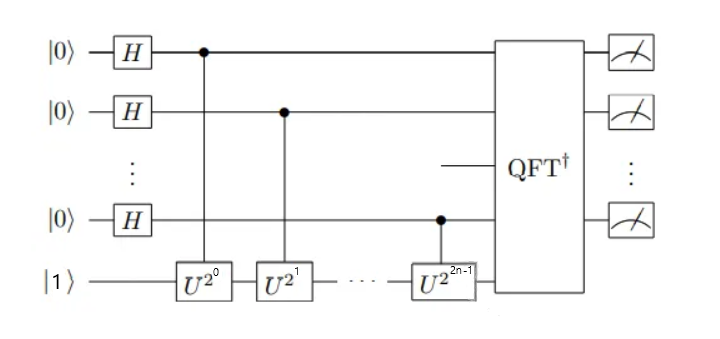
\includegraphics[width=\columnwidth]{shor_n_qubit.png}
    \centering
    \end{figure}

Die Realisierung der Transformation bedingt die Implementierung einiger arithmetischer Operationen in Form eines Quantenschaltkreises. 
Diese fungieren als Bausteine, die zusammengesetzt zur Konstruktion des übergeordneten Quantenschaltkreises für die modulare Multiplikation beitragen. 
Zu den erforderlichen arithmetischen Operationen gehört die Addition, Subtraktion sowie die modulare Addition.

In den folgenden Abschnitten werden die untergeordneten arithmetischen Operationen bis hin zur modularen Multiplikation implementiert.

\subsubsection{Addition}
Der Quantenschaltkreis für die Addition bildet das Fundament der \(U\)-Gatter und 
stellt einen der am häufigsten verwendeten Bausteine dar. 
Deswegen hat die Implementierung der Addition einen erheblichen Einfluss auf den Ressourcenbedarf des gesamten Quantenalgorithmus
und sollte daher möglichst effizient implementiert werden.

Eine Möglichkeit, die Addition als Quantenschaltkreis zu realisieren, 
besteht im Nachbau eines klassischen Schaltkreises aus Volladdierern. 
Da es nicht möglich ist, 
die notwendige klassischen Gatter wie AND und OR als unitäre Transformation mit nur zwei Qubits darzustellen~\cite{Hoever2023QC},
werden zusätzliche Hilfsqubits benötigt.
Die zusätzlichen Hilfsqubits bewirken, dass der Nachbau eines klassischen Schaltkreis für die Addition zweier \(n\)-Bit Zahlen, 
also solche der Größenordnung \(2^n\), mindestens \(3n\) Qubits benötigt~\cite{zalka1998fast}.

Eine effizientere Methode, die ohne Hilfsqubits auskommt, ist die Quanten-Addition~\cite{draper2000addition}. 
Die Quanten-Addition führt die Berechnung auf quantenmechanische Weise durch. 
Im Wesentlichen wird dabei die Addition in der Fourier-Basis berechnet, 
wobei die Phasen der Qubits eines Summanden mit kontrollierte Phasenverschiebungen auf die Qubits des anderen Summanden wirkt.

Im Folgenden wird ein Beispiel für die Quanten-Addition zweier Qubit-Register \(\ket{a}_3\) und \(\ket{b}_3\), 
jeweils bestehend aus drei Qubits, betrachtet:
\begin{figure}[H]
    \caption{Quantum-Addition}
    \label{fig:3_qubit_quantum_add}
    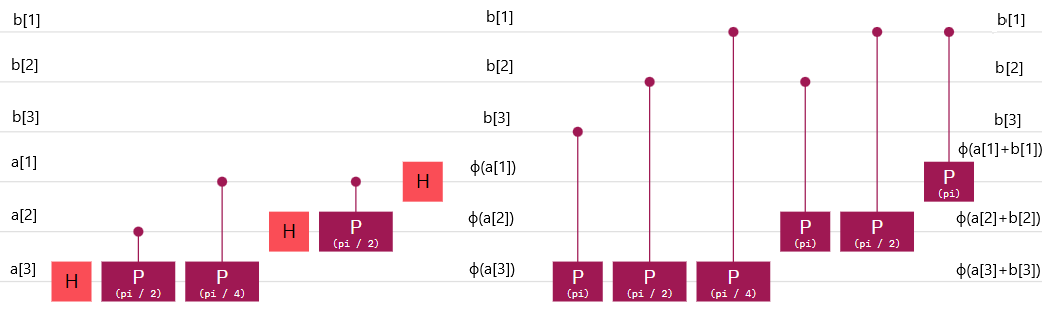
\includegraphics[width=\columnwidth]{3_qubit_quantum_add.png}
    \centering
    \end{figure}
Die Registermarkierungen in der Mitte von Abbildung~\ref*{fig:3_qubit_quantum_add} unterteilen die Darstellung in zwei Hälften.
Die linke Hälfte repräsentiert die Quanten-Fourier-Transformation, 
während die rechte Hälfte die Quanten-Addition zeigt.

Wie man an der Struktur der Quanten-Addition erkennen kann,
ist die Anordnung der Gatter fast identisch mit der Quanten-Fourier-Transformation.
Ein Unterschied besteht darin, 
dass die Hadamard-Gatter durch kontrollierte \(P(\pi)\) Phasen-Gatter ersetzt wurden.
Sowohl das Hadamard-Gatter als auch das \(P(\pi)\) Phasen-Gatter erzeugen eine relative Phase von \(e^{\pi i}\).
Ein weiterer Unterschied zur Quanten-Fourier-Transformation besteht darin, 
dass die Phasen-Gatter nicht durch das gleiche Register\(\ket{a}_3\) kontrolliert werden, 
auf das die Gatter auch wirken.
Stattdessen kontrollieren die Qubits des Registers \(\ket{b}_3\) die Phasen-Gatter.
Dabei wird das \(P(\pi)\) Phasen-Gatter durch das Qubit des \(\ket{b}_3\) kontrolliert,
welches die selbe Wertigkeit hat wie das Zielqubit des \(\ket{a}_3\) Registers.
Jedes weitere kontrollierte Phasen-Gatter für das gleiche Zielqubit 
wird fortlaufend von dem nächstkleineren Qubit von \(\ket{b}_3\) kontrolliert.

Im Prinzip handelt es sich bei dieser Quantenschaltung um eine Anwendung derselben Phasenverschiebungen 
wie bei der Quanten-Fourier-Transformation. 
Der grundlegende Unterschied liegt darin, 
dass diese Phasenverschiebungen kontrolliert auf ein anderes Quantenregister angewendet werden.

Die Wirkung der Quanten-Addition wird anhand der Abbildung~\ref*{fig:3_qubit_quantum_add} verdeutlicht:
Am Anfang der linken Hälfte befinden sich beide Register in der Standardbasis.
Auf das Zielregister \(\ket{a}_3\) wirkt die Quanten-Fourier-Transformation ohne Swap Gatter.
Dadurch befindet sich \(\ket{a}_3\) nun in der Fourier-Basis \(\Phi\), also \(\ket{\Phi(a)}_3\):
\[\ket{\Phi(a)}_3 = \frac{1}{\sqrt{8}} [ (\ket{0} + { e^{\frac{2 \pi i (2^0a_1)}{2^1}}}\ket{1} ) \bigotimes
( \ket{0} + { e^{\frac{2 \pi i (2^1a_2+2^0a_1)}{2^2}}}\ket{1} ) \bigotimes
( \ket{0} + { e^{\frac{2 \pi i (2^{2}a_3 +2^1a_2+2^0a_1)}{2^3}}}\ket{1} ) ] \]
Anschließend wirkt auf das hinterste Tensorprodukt ein \(P(\pi)\) Phasen-Gatter,
welches durch \(\ket{b_3}_1\) kontrolliert wird.
Wenn sich \(\ket{b_3}_1\) im Zustand \(\ket{0}_1\) befindet, passiert nichts.
Wenn es sich im Zustand \(\ket{1}_1\) befindet, dass das Phasen-Gatter angewendet wird.
Dieses Verhalten kann man für beide Fälle mit den entsprechenden Matrizen 
\(\begin{pmatrix}
    1 & 0 \\
    0 & e^{\pi i b_3}
  \end{pmatrix}\)
  beziehungsweise  
  \(\begin{pmatrix}
    1 & 0 \\
    0 & e^{\frac{2\pi i (2^2b_3)}{2^3}}
  \end{pmatrix}\)
beschreiben.
Schreibt man das hinterste Tensorprodukt als Vektor, ergibt sich die folgende Formulierung:
\[\frac{1}{\sqrt{2}}( \ket{0} + { e^{\frac{2 \pi i (2^{2}a_3 +2^1a_2+2^0a_1)}{2^3}}}\ket{1}) \equiv
\frac{1}{\sqrt{2}}
\begin{pmatrix}
     1  \\
     e^{\frac{2 \pi i (2^{2}a_3 +2^1a_2+2^0a_1)}{2^3}}
  \end{pmatrix}
    \]
Dann wird durch das Ergebnis der Verrechnung mit dem Phasen-Gatter deutlich, 
dass die Addition im Wesentlichen in der Phase des Quantenzustands stattfindet:
\[\begin{pmatrix}
    1 & 0 \\
    0 & e^{\frac{2\pi i (2^2b_3)}{2^3}}
  \end{pmatrix}
    \cdot
\frac{1}{\sqrt{2}}
\begin{pmatrix}
    1  \\
     e^{\frac{2 \pi i (2^{2}a_3 +2^1a_2+2^0a_1)}{2^3}}
  \end{pmatrix}
  =
  \frac{1}{\sqrt{2}}
  \begin{pmatrix}
    1  \\
     e^{\frac{2 \pi i (2^{2}(a_3+b_3) +2^1a_2+2^0a_1)}{2^3}}
  \end{pmatrix}
\]
Wie in der Abbildung~\ref*{fig:3_qubit_quantum_add} erkenntlich,
wirken auf das hinterste Tensorprodukt auch noch die beiden Phasen-Gatter \(P(\frac{\pi}{2})\) und \(P(\frac{\pi}{4})\) mit:
\[
    P(\frac{\pi}{2}) = 
\begin{pmatrix}
    1 & 0 \\
    0 & e^{\frac{\pi}{2} i b_2}
  \end{pmatrix}
  =
  \begin{pmatrix}
    1 & 0 \\
    0 & e^{\frac{2\pi i (2^1b_2)}{2^3}}
  \end{pmatrix}
  ~;~
P(\frac{\pi}{4}) = 
\begin{pmatrix}
    1 & 0 \\
    0 & e^{\frac{\pi}{4} i b_1}
  \end{pmatrix}
  =
  \begin{pmatrix}
    1 & 0 \\
    0 & e^{\frac{2\pi i (2^0b_1)}{2^3}}
  \end{pmatrix}
\]
\[
    \begin{pmatrix}
        1 & 0 \\
        0 & e^{\frac{2\pi i (2^0b_1)}{2^3}}
      \end{pmatrix}
      \cdot
      \begin{pmatrix}
        1 & 0 \\
        0 & e^{\frac{2\pi i (2^1b_2)}{2^3}}
      \end{pmatrix}
      \cdot
      \frac{1}{\sqrt{2}}
      \begin{pmatrix}
        1  \\
         e^{\frac{2 \pi i (2^{2}(a_3+b_3) +2^1a_2+2^0a_1)}{2^3}}
      \end{pmatrix}
      =
      \frac{1}{\sqrt{2}}
      \begin{pmatrix}
        1  \\
         e^{\frac{2 \pi i (2^{2}(a_3+b_3) +2^1(a_2+b_2)+2^0(a_1+b_1))}{2^3}}
      \end{pmatrix}
\]
Wendet man alle weiteren Phasen-Gatter auf das vollstände Tensorprodukt an, 
erhält man:
\[
    \frac{1}{\sqrt{8}} [ (\ket{0} + { e^{\frac{2 \pi i (2^0(a_1+b_1))}{2^1}}}\ket{1} ) \bigotimes
( \ket{0} + { e^{\frac{2 \pi i (2^1(a_2+b_2)+2^0(a_1+b_1))}{2^2}}}\ket{1} ) \bigotimes
( \ket{0} + { e^{\frac{2 \pi i (2^{2}(a_3+b_3) +2^1(a_2+b_2)+2^0(a_1+b_1))}{2^3}}}\ket{1} ) ]
\]
Setzt man in diese Formel zwei Zahlen in Binärschreibweise ein, 
wird man den selben Zustand erhalten,
wie wenn man die Summe der beiden Zahlen in die Formel der Quanten-Fourier-Transformation einsetzt.
Beispielsweise sei \(a = 3\) also binär \(a_3 = 0\), \(a_2 = 1\),\(a_1 = 1\) und 
\(b = 1\) also \(b_3 = 0\), \(b_2 = 0\),\(b_1 = 1\):
\[
\frac{1}{\sqrt{8}} [ (\ket{0} + { e^{\frac{2 \pi i (2^0(1+1))}{2^1}}}\ket{1} ) \bigotimes
( \ket{0} + { e^{\frac{2 \pi i (2^1(1+0)+2^0(1+1))}{2^2}}}\ket{1} ) \bigotimes
( \ket{0} + { e^{\frac{2 \pi i (2^{2}(0+0) +2^1(1+0)+2^0(1+1))}{2^3}}}\ket{1} ) ]
\]
\[
=\frac{1}{\sqrt{8}} [ (\ket{0} + \ket{1} ) \bigotimes
( \ket{0} +   \ket{1} ) \bigotimes
( \ket{0} +  e^{\pi i }\ket{1} ) ]
\]
Das dies tatsächlich die Summe in Fourier-Basis entspricht, 
wird deutlich wenn man das selbe Tensorprodukt aus der Quanten-Fourier-Transformation bildet:
\[
    QFT(\ket{c}_3)
    \frac{1}{\sqrt{8}} [ (\ket{0} + { e^{\frac{2 \pi i (2^0(c_1))}{2^1}}}\ket{1} ) \bigotimes
( \ket{0} + { e^{\frac{2 \pi i (2^1(c_2)+2^0(c_1))}{2^2}}}\ket{1} ) \bigotimes
( \ket{0} + { e^{\frac{2 \pi i (2^{2}(c_3) +2^1(c_2)+2^0(c_1))}{2^3}}}\ket{1} ) ]
\]
Die Summe von \(a\) und \(b\) entspricht \(c = 4\) also \(c_3 = 1,~c_2 = 0,~c_1=0\):
\[
    QFT(\ket{4}_3)
    \frac{1}{\sqrt{8}} [ (\ket{0} + { e^{\frac{2 \pi i (2^0(0))}{2^1}}}\ket{1} ) \bigotimes
( \ket{0} + { e^{\frac{2 \pi i (2^1(0)+2^0(0))}{2^2}}}\ket{1} ) \bigotimes
( \ket{0} + { e^{\frac{2 \pi i (2^{2}(1) +2^1(0)+2^0(0))}{2^3}}}\ket{1} ) ]
\]
\[
    = 
    \frac{1}{\sqrt{8}} [ (\ket{0} + { e^{\frac{2 \pi i (0)}{2^1}}}\ket{1} ) \bigotimes
( \ket{0} + { e^{\frac{2 \pi i (0)}{2^2}}}\ket{1} ) \bigotimes
( \ket{0} + { e^{\frac{2 \pi i (2^{2}(1))}{2^3}}}\ket{1} ) ]
\]
\[
=\frac{1}{\sqrt{8}} [ (\ket{0} + \ket{1} ) \bigotimes
( \ket{0} +   \ket{1} ) \bigotimes
( \ket{0} +  e^{\pi i }\ket{1} ) ]
\]
Das Ergebnis der Quanten-Addition zweier Summanden \(a=3,~b=1\), 
jeweils in einem Register mit drei Qubits,
ist somit identisch mit dem Zustand, 
der durch die Anwendung der Quanten-Fourier-Transformation auf ein Register 
aus ebenfalls drei Qubits mit der Summe der beiden Zahlen entsteht.

Mit einer anschließenden inversen Quanten-Fourier-Transformation, 
kann die Summe in die Standardbasis und somit in einen Messbaren Zustand transformiert werden:
\[
iQFT(\ket{\Phi(4)_3})
\equiv
 iQFT(\frac{1}{\sqrt{8}} [ (\ket{0} + \ket{1} ) \bigotimes
( \ket{0} +   \ket{1} ) \bigotimes
( \ket{0} +  e^{\pi i }\ket{1} ) ]) 
=
\ket{4}_3
\]

Für die Realisierung der modularen Multiplikation wird zu keinem Zeitpunkt der Berechnung eine Addition zweier Zwischenergebnisse benötigt. 
Genauer gesagt, ist es nicht nötig, ein Quantenregister auf ein anderes zu addieren. 
Stattdessen wird die Quanten-Addition benutzt, um eine vorab bekannte Zahl auf ein Quantenregister zu addieren.

Bei der Quanten-Addition mit zwei Register wie in Abbildung~\ref*{fig:3_qubit_quantum_add} erfolgt die Phasenverschiebung kontrolliert,  
also in Abhängigkeit des Inhaltes von Register \(\ket{b}_3\).
Ist der Inhalt von Register \(\ket{b}_3\) vorab bekannt,
können gewöhnliche Phasen-Gatter anstelle von kontrollierten verwendet werden~\cite*{beauregard2003circuit}.

Wenn bei der Quanten-Addition mit zwei Registern ein Phasen-Gatter aufgrund des zugehörigen Kontrollqubits im Zustand \(\ket{1}\) angewendet wird,
wird es in der Variante mit einem einzelnen Register als gewöhnliches Phasen-Gatter verwendet.
Ist das Kontrollqubit hingegen im Zustand \(\ket{0}\), 
wodurch das Phasen-Gatter bei der Quanten-Addition mit zwei Registern nicht zur Anwendung kommt, 
wird dieses Phasen-Gatter in der Variante mit nur einem Register weggelassen.

\begin{figure}[H]
    \caption{Quantum-Addition fixierte Phasenverschiebungen}
    \label{fig:3_qubit_fixed_quantum_addition}
    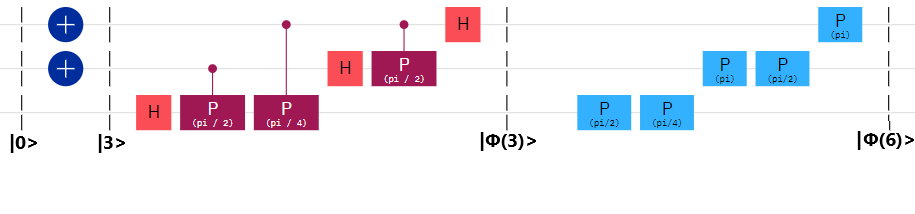
\includegraphics[width=\columnwidth]{3_qubit_fixed_quantum_addition.png}
    \centering
    \end{figure}
In Abbildung~\ref*{fig:3_qubit_fixed_quantum_addition} ist die Quanten-Addition für ein 3-Qubit Register abgebildet.
Die blauen Phasen-Gatter sorgen für die Quanten-Addition mit einem fixierten Wert von \(3\).
Vergleicht man die Abbildung~\ref*{fig:3_qubit_fixed_quantum_addition} mit der Abbildung~\ref*{fig:3_qubit_quantum_add} fällt auf, 
dass das aller erste Phasen-Gatter der Quanten-Addition nicht vorkommt.
Im Quantenschaltkreis der Abbildung~\ref*{fig:3_qubit_quantum_add} würde ein Registerinhalt von \(b = 3\) das Kontrollqubit \(b_3\) nicht setzen. 
Somit kommt das erste Phasen-Gatter der Quanten-Addition nicht zum Einsatz und 
wird deswegen in der Variante aus Abbildung~\ref*{fig:3_qubit_fixed_quantum_addition} weggelassen. 









